\documentclass[fontsize=12pt]{article}
\oddsidemargin=-1cm
\textwidth=18cm
\textheight=20cm
\setlength{\parindent}{10mm}
\setlength{\parskip}{0.9em}
\def\baselinestretch{1.5}

\usepackage[spanish]{babel}
\renewcommand {\spanishtablename}{Tabla}
\usepackage[utf8]{inputenc}
\usepackage{graphicx}
\usepackage{caption} 
\usepackage{amsmath, amsthm, amsfonts}
\usepackage{enumerate} 
\usepackage{fancyhdr}
\usepackage{anysize} 
\usepackage[usenames]{color}
\usepackage{booktabs}


\lhead{\begin{picture}(0,0) \put(0,0){\includegraphics[width=40mm]{./uanl.jpg}} \end{picture}}
\chead{\vspace{-0.3cm} \begin{tabular}[l]{@{}l@{}l@{}}Nombre: Johanna Bolaños Zúñiga\\ Matricula: 1883900 \\ Modelos Probabilistas Aplicados \end{tabular} \vspace{0.01cm}}
\rhead{\begin{picture}(115,0) \put(0,0){\includegraphics[width=42mm]{./pisis.png}} \end{picture}}
\renewcommand{\headrulewidth}{0.6pt}

\pagestyle{fancy}

\begin{document}

%\newpage
%\tableofcontents 
%\newpage

\textcolor[rgb]{1,1,1}{-}
\begin{center}
\Large \textbf{Tarea 1}
\end{center}


\section{Recopilación de datos - Sección Precios} \label{recopdedatos}

En el presente trabajo se realiza un análisis estadístico con el programa R versión 4.0.2. Se utilizó la información del Índice Nacional de Precios al Consumidor (INPC) \footnote{El INPC es un indicador económico que muestra la variación de los precios en un periodo de tiempo.} mensual por ciudades en el periodo de enero 2019 - 2020. Esta información fue consultada en la página del INEGI \cite{INEGI}, en la sección de Precios.

La información de las 55 ciudades del INPC y su respectivo índice con base en la segunda quincena de julio 2018, fueron descargadas en un archivo .xlsx. Para efectos del estudio, se filtró la información de las 3 principales ciudades de México (Monterrey, Ciudad de México y Guadalajara ), la cual se muestra en la Tabla \ref{datos}. Estos datos se guardaron en un archivo .dat. 


\begin{table}[htp]
\centering
\caption{Índice Nacional de Precios al Consumidor}
\label{datos}
\begin{tabular}{|l|c|c|c|}
\hline
\multicolumn{1}{|c|}{\textbf{Fecha}} & \textbf{Monterrey} & \multicolumn{1}{c|}{\textbf{\begin{tabular}[c]{@{}c@{}}Ciudad\\ De México\end{tabular}}} & \textbf{Guadalajara} \\ \hline
Ene 2019                             & 103.548            & 102.653                                                                                  & 102.078              \\ \hline
Feb 2019                             & 103.791            & 102.513                                                                                  & 102.468              \\ \hline
Mar 209                              & 104.090            & 102.859                                                                                  & 103.275              \\ \hline
Abr 2019                             & 102.993            & 103.291                                                                                  & 103.646              \\ \hline
May 2019                             & 102.945            & 103.523                                                                                  & 103.827              \\ \hline
Jun 2019                             & 102.998            & 103.741                                                                                  & 103.893              \\ \hline
Jul 2019                             & 103.762            & 104.079                                                                                  & 103.993              \\ \hline
Ago 2019                             & 103.814            & 103.817                                                                                  & 104.003              \\ \hline
Sep 2019                             & 104.038            & 104.134                                                                                  & 104.124              \\ \hline
Oct 2019                             & 105.636            & 104.372                                                                                  & 104.543              \\ \hline
Nov 2019                             & 105.892            & 104.952                                                                                  & 105.060              \\ \hline
Dic 2019                             & 106.301            & 105.659                                                                                  & 105.764              \\ \hline
Ene 2020                             & 106.793            & 106.060                                                                                  & 105.805              \\ \hline
\end{tabular}
\end{table}


\section{Diagrama de cajas y bigotes}
Para realizar el análisis estadístico y como ayuda visual para identificar el comportamiento de los datos de la sección \ref{recopdedatos}, se utilizó el diagrama de cajas y bigotes. El código en R se encuentra en el repositorio github.com/JohannaBZ/Probabilidad/tree/master/Tarea\%201

De acuerdo a la Figura \ref{PrincipalesCiudades} podemos observar que, entre las 3 ciudades principales de México, el INPC más bajo lo reportó Guadalajara y el más alto lo registró Monterrey, mientras que, Ciudad de México registró una variación atípica. También se puede observar que la mediana de los INPC de las tres ciudades es muy similar, aunque Monterrey registró una mayor variabilidad, mantuvo por más tiempo INPC bajos, sin embargo, Guadalajara mantuvo por más tiempo los INPC altos.


\begin{figure}[htp]
\centering
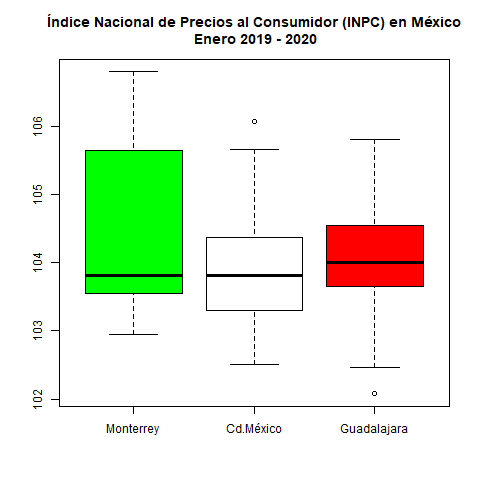
\includegraphics[scale=0.8]{PrincipalesCiudades}
\caption{Índice Nacional de Precios al Consumidor de enero 2019 - 2020 en las 3 ciudades principales de México}
\label{PrincipalesCiudades}
\end{figure}

De igual forma, en la Figura \ref{TotalCiudades} se muestran los índices de las 55 ciudades del INPC reportadas por la INEGI, en la cual podemos observar que el INPC más alto lo reportó Hermosillo y el más bajo fue en Tijuana. También se puede observar que varias ciudades registraron variaciones atípicas en el INPC.

\begin{figure}[h]
\centering
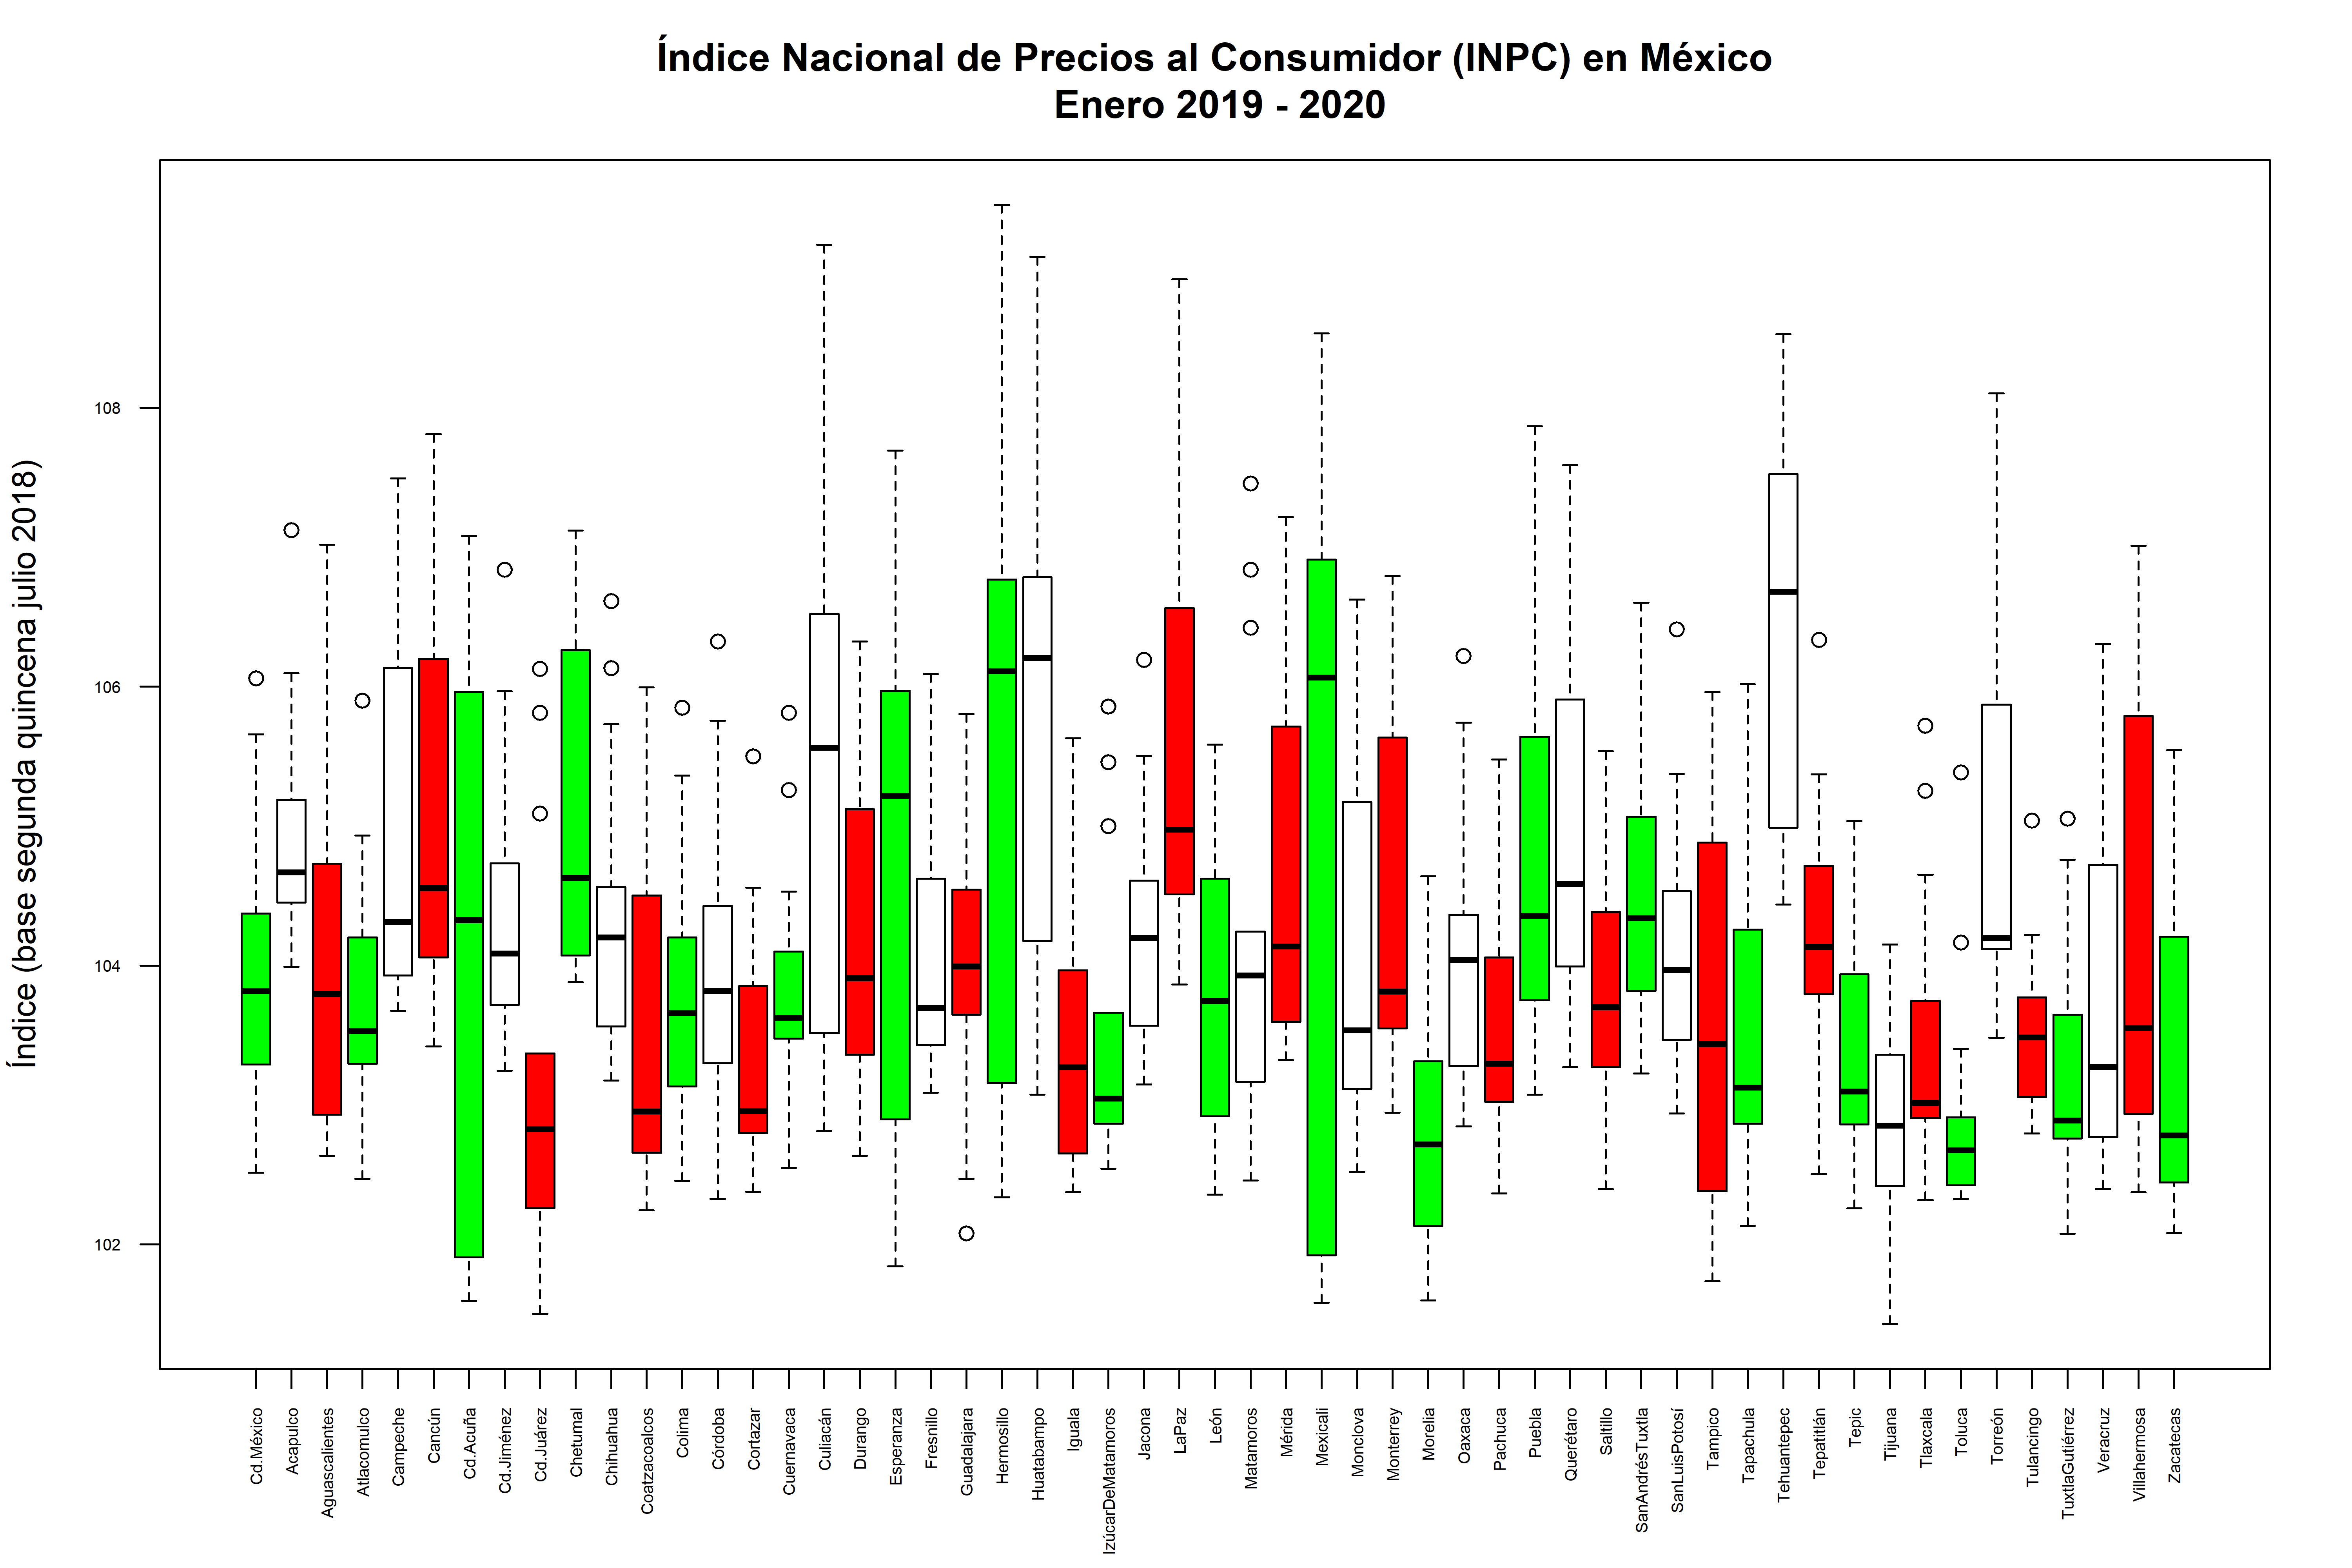
\includegraphics[scale=0.55]{TotalCiudades}
\caption{Índice Nacional de Precios al Consumidor de enero 2019 - 2020 en las 55 ciudades del INPC en México}
\label{TotalCiudades}
\end{figure}


\bibliography{MiBiblio}
\bibliographystyle{plain}
	
	
	
	

\end{document}
